\section{Theory \& Simulation}
The purpose of the simulations were to identify what the main signal processing factors are when producing a directional audio system. To do so, the audible signal had to be generated, passed through the inverse transfer function of the environment defined by Berktay's approximation shown in equation \ref{eqn:berktayRelationship} and finally applied to the approximate transfer function of the environment along with appropriate filtering to mimic the human hearing range. The outcome from these simulations would show what factors were important in the synthesis of a directional ultrasonic beam and the audible demodulation of said beam. All signal simulations were done in Julia \cite{bezanson2017julia} with aid from the FFTW\cite{Padua2011} Julia standard libraries.
\subsection{Signal generation}
During initial simulations a 1kHz tone denoted by $x(t)$ and a carrier signal at 40kHz defined as $x_{cw}(t)$ were generated. $x(t)$ was chosen to be a sine wave while $x_{cw}(t)$ was set as a cosine function to simplify the mathematics involved. Both signals were then passed into the signal pre-processing stage of the simulation.
\begin{equation}
    x(t) = sin(\omega_0 t)
\end{equation}
\begin{equation}
    x_{cw}(t) = cos(\omega_c t)
\end{equation}
The 1kHz tone and carrier signal are denoted by $\omega_0$ and $\omega_c$ respectively.

\subsection{Pre-processing}
To achieve an audible signal in the environment, the inverse function of the environment must be applied to the signal prior to transmission. Berktay's approximation \cite{berktay_1965} shown in equation \ref{eqn:berktayRelationship}, has the following inverse shown below in equation \ref{eqn:inverseBerk}.
\begin{equation}
    p_{out}(t) = \iint \sqrt{p_1(t)} dt^2
    \label{eqn:inverseBerk}
\end{equation}
$p_1(t)$ represents the pressure wave to be heared in the environment. By applying the second time integral to the square root of the original waveform, the environment will apply its second time derivative to the square of the output function ($p_{out}(t)$) resulting in the original audible pressure waves as shown below in equation \ref{eqn:inverseApply} and \ref{eqn:p2=p1}.
\begin{equation}
        p_2(t) \approx \frac{\partial^2}{\partial t^2}\left(\iint \sqrt{p_1(t)} dt^2\right)^2
        \label{eqn:inverseApply}
\end{equation}
\begin{equation}
        p_2(t) \approx p_1(t)
        \label{eqn:p2=p1}
\end{equation}
Implementing this type of signal processing in the simulation was done on a discrete sample by sample level to allow for easier adaptability of any processing factors that may arise. The double integration of the signal was done by use of a simple left sided Riemann sum shown in listing \ref{lst:integrate}. For each result, the input signals value is multiplied by sample period ($\Delta t$) and then added to the previous result of the integral. Edge cases were handled by starting at the second sample and assuming the integral starts at the origin.
\begin{lstlisting}[caption={Left sided integration function written in Julia}\label{lst:integrate},language=julia, style=jlcodestyle]
function integrate(x, Δt)
    y=zeros(length(x));
    N = length(x)
    for n=2:N
        y[n]=x[n-1]*Δt + y[n-1]
    end
    return y
end
\end{lstlisting}
With each integration, the mean of the signal is subtracted from the the original signal to correct the signal back to the origin as shown in listing \ref{lst:meanshift}. This shift is necessary as the drift in signal level limits its ability to be produced out of a real transducer.
\begin{lstlisting}[caption={Shifting signal to its average value before integration}\label{lst:meanshift},language=julia, style=jlcodestyle]
#Pre-process signal             
y'=integrate(x.-mean(x),Δt)     #perform first integral of the audio signal
y''=integrate(y'.-mean(y'),Δt)   #perform second integral of the audio signal
\end{lstlisting}

Following the integration steps, the absolute value of the signal is determined and the square root applied, shown in listing \ref{lst:squaring}. The absolute value is necessary as the square root of the negative samples would yield an imaginary result which cannot practically be reproduced in the real world implementation. The signal is finally modulated with a 40kHz carrier wave for transmission into the simulated medium.

\begin{lstlisting}[caption={Take absolute value of integrated signal and apply the square root}\label{lst:squaring},language=julia, style=jlcodestyle]
y'' = y''.-minimum(y'')           #shifts the signal to above 0
yout = y''.^(1/2)               #Square root the signal
yout_mod = yout.*x_carrier        #Modulate the preprocessed signal with carrier
\end{lstlisting}

\subsection{Environment transfer function simulation}
The pre-processed signal is now applied to the environment's transfer function by applying the mathematical operations shown in equation \ref{eqn:berktayRelationship}. The first operation which is applied is the squaring of the pre-processed signal. This is done by taking the square of each sample with the use of the power operator in julia. This squared signal is then transformed to its Fourier transformed representation so a FIR filter can be applied. The filter construction is shown in listing \ref{lst:FIRfilter} and forms a tophat function from -15kHz to 15kHz to filter out any signals outside of the band of human hearing.

\begin{lstlisting}[caption={FIR filter for mimicing human hearing }\label{lst:FIRfilter},language=julia, style=jlcodestyle]
Δω = 2*pi/(N*Δt)  # Sample spacing in freq domain in rad/s
ω = 0:Δω:(N-1)*Δω # Define angular frequency 
B = 30000 # filter bandwidth of 30KHz to span from -15 to 15 KHz
H = rect.(ω/(2*pi*B)) + rect.( (ω .- 2*pi/Δt)/(2*pi*B) ) #Tophat = __|----|__
Hs=[i[1] for i in H]# Change array type so iFFT works

#transform function into frequency domain
YOUT_sqr = fft(yout_mod_sqr)
#Apply filter
YOUT_sqr_LPF = YOUT_sqr.*Hs
\end{lstlisting}

Application of the filter is done by multiplying the Fourier representations of the filter with the signal shown in the lower portion of listing \ref{lst:FIRfilter}.\\

The signal is then transformed back into the time domain for the last stage of signal processing. The double time derivative of the time domain expression is then applied to account for the $\frac{\partial}{\partial t}$ of equation \ref{eqn:berktayRelationship}. Additionally the time domain expression is multiplied by 2 to account for the halving of the signal when taking only the real parts of a inverse Fourier transform. Listing \ref{lst:doubledt} shows the implementation of the inverse Fourier transform and double derivatives in julia. The \texttt{deriv()} function is defined in listing \ref{lst:deriv} which applies a left sided derivitive to each sample much like the integral defined in listing \ref{lst:integrate}.

\begin{lstlisting}[caption={derivative function implementing a sample wise left sided derivative}\label{lst:deriv},language=julia, style=jlcodestyle]
function deriv(x,Δt)
    y=zeros(length(x))
    N = length(x)
    for n=2:N
       y[n]=(x[n]-x[n-1])/Δt
    end
    return y
end
\end{lstlisting}

The \texttt{shiftBackBy()} function is a function which shifts a sampled signal back by a number of samples. Its purpose is to remove the artifacts that occur during the sample wise differentiation. These artifacts occur due to the initial value of the signal being set to 0 during differentiation. A shift of a single sample would not be noticeable to human hearing and thus should not be considered an issue for the system as a whole. The code for this shifting function is shown in listing \ref{lst:shift}
\begin{lstlisting}[caption={Function for shifting sampled signal back by a set number of samples}\label{lst:shift},language=julia, style=jlcodestyle]
function shiftBackBy(x,shift)
    yshift=zeros(length(x))
    N = length(x)
    for n=1:N-shift
        yshift[n]=x[n+shift]
    end
    return yshift
end
\end{lstlisting}

\begin{lstlisting}[caption={Conversion to time domain and double time derivative}\label{lst:doubledt},language=julia, style=jlcodestyle]

yout_mod_sqr_lpf = 2*real(ifft(YOUT_sqr_LPF))   #Extract  time-domain

yout_mod_sqr_dt1_lpf = deriv(yout_mod_sqr_lpf,Δt)   #Differentiate signal once
yout_mod_sqr_dt1_lpf = shiftBackBy(yout_mod_sqr_dt1_lpf,1)
yout_mod_sqr_dt2 = deriv(yout_mod_sqr_dt1_lpf,Δt)   #Differentiate signal again
yout_mod_sqr_dt2 = shiftBackBy(yout_mod_sqr_dt2,1)
\end{lstlisting}

The final signal \texttt{yout\_mod\_sqr\_dt2} is the time domain expression of the audio signal after it has passed through the environment simulation.

\newpage
\subsection{Simulation results and discussion}
The results for major parts in the signal chain from the simulations will be presented here and discussed.
\subsubsection{Pre-processing}
During pre-processing, the signal undergoes a double integral. The time domain representation of the signal after the first and second integrals is shown in figure \ref{fig:tdomint12}. The positive frequency domain representation of the first and second integral are shown in figure \ref{fig:fdomint12}.

\begin{figure}[ht!]
    \centering
    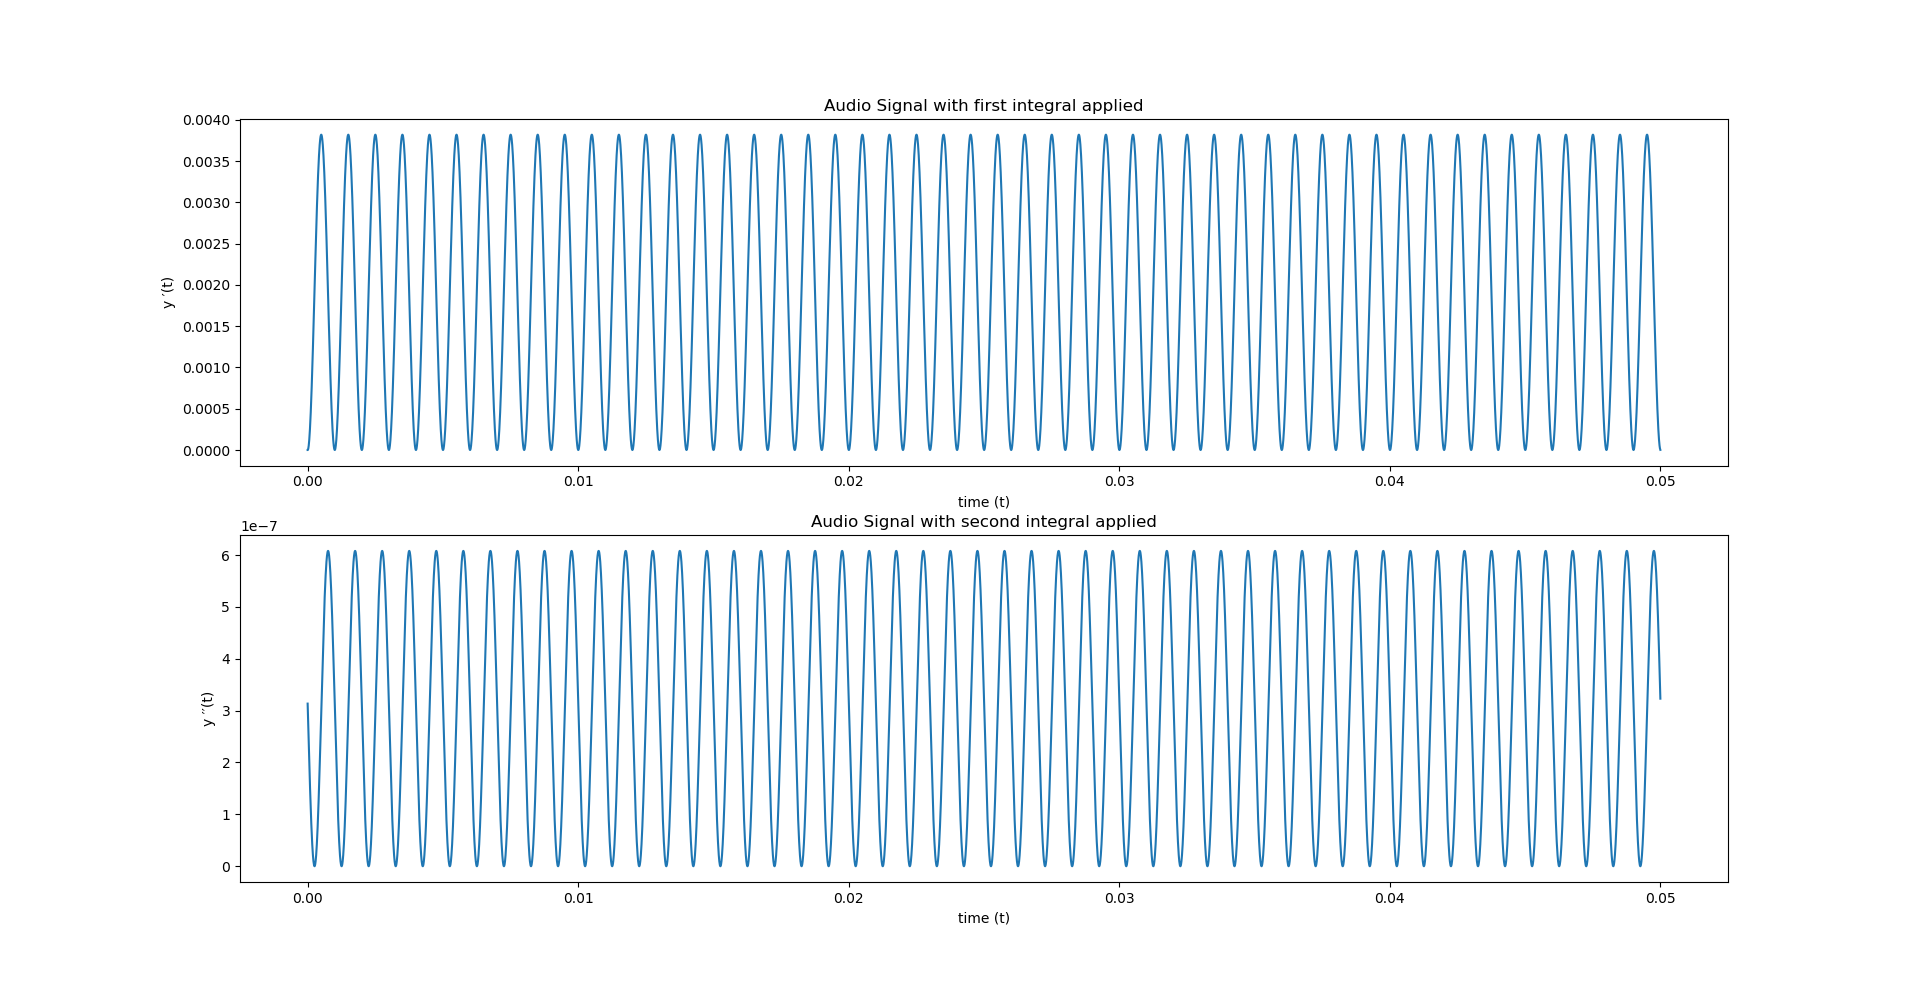
\includegraphics[width=0.8\textwidth]{Figures/SigSimulation/simint1int2.png}
    \caption{The time domain representation of the 1 kHz signal after the first and second integral}
    \label{fig:tdomint12}
\end{figure}
\begin{figure}[ht!]
    \centering
    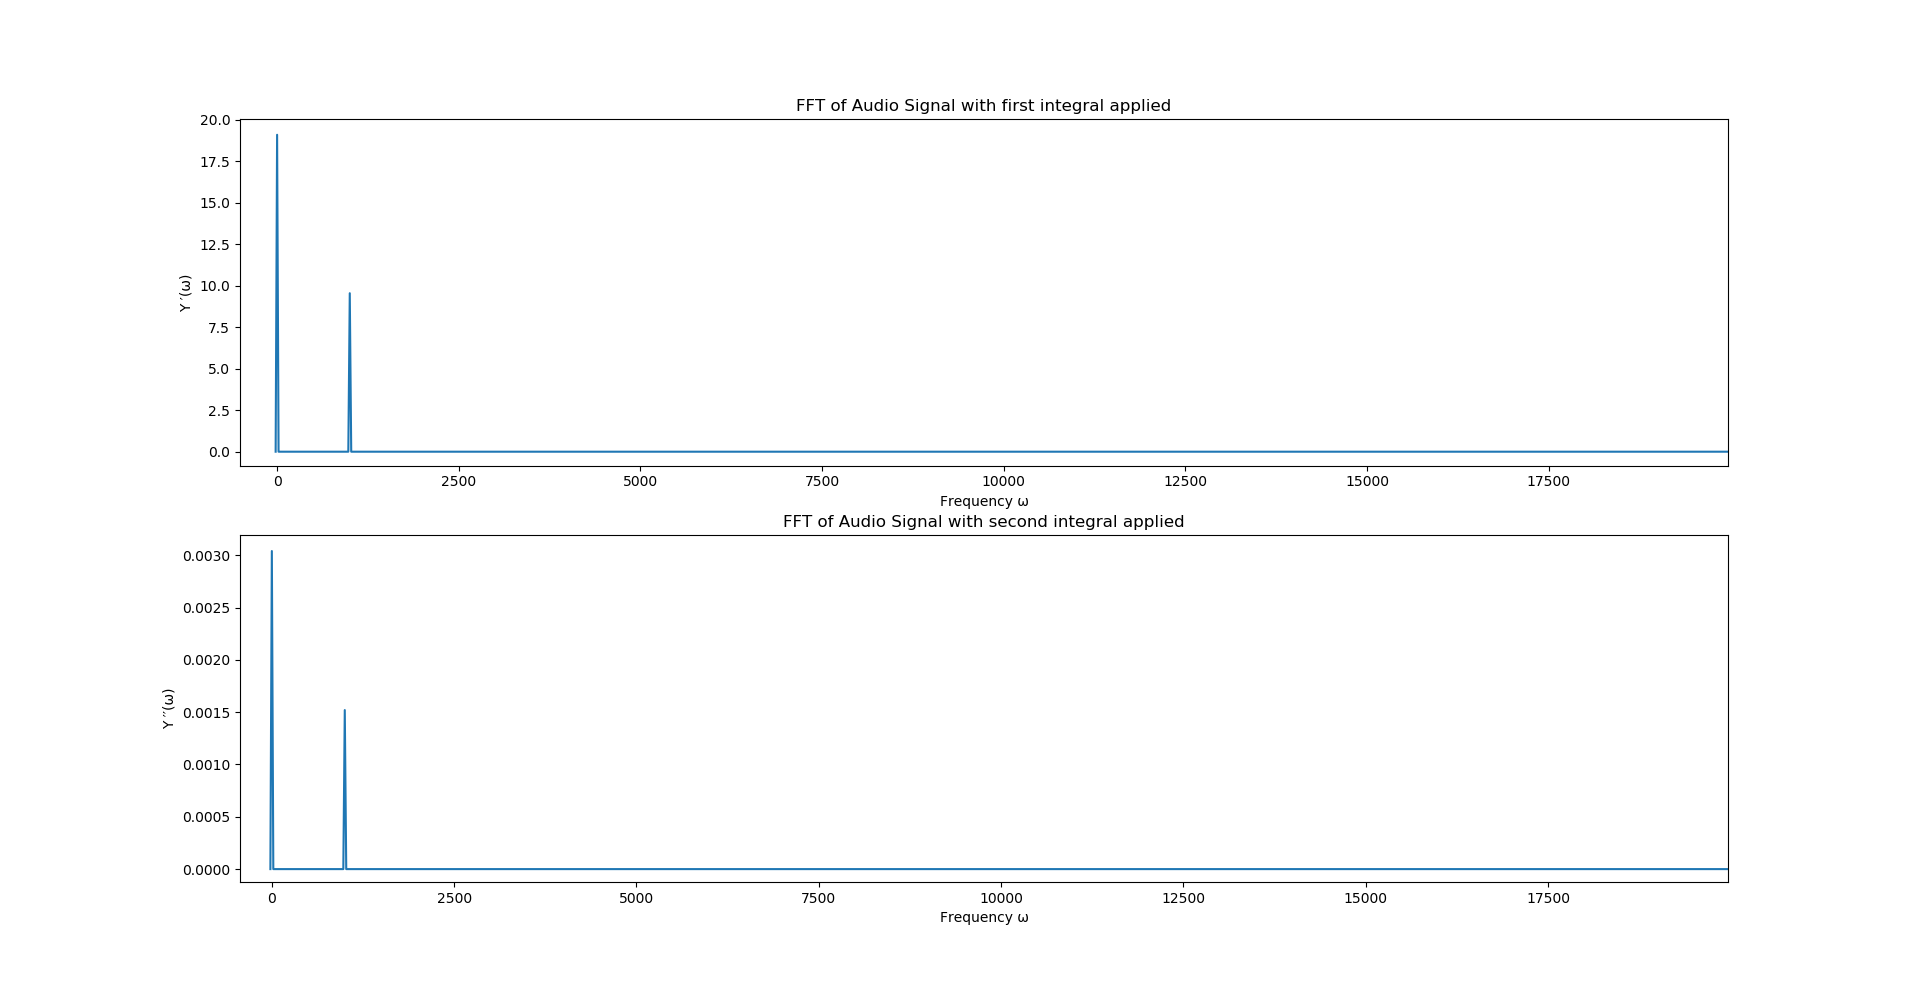
\includegraphics[width=0.8\textwidth]{Figures/SigSimulation/fftsimint1int2.png}
    \caption{The frequency domain representation of the 1 kHz signal after the first and second integral}
    \label{fig:fdomint12}
\end{figure}
\newpage
The only notable difference between these results is the decrease in amplitude of the sine wave as well as a phase shift of about $90^\circ$ between the time domain representations in figure \ref{fig:tdomint12}. This phase shift is expected since the integral of a sinusoidal function produces another sinusoidal function with a phase shift.\\

Moving forward within the pre-processing chain, the result of these integrals is then square-rooted according to the code shown in listing \ref{lst:squaring}. This results in decaying harmonics as shown in figure \ref{fig:sqrtsimmodfft} which are then modulated with the 40 kHz carrier signal through AM modulation.
\begin{figure}[ht!]
    \centering
    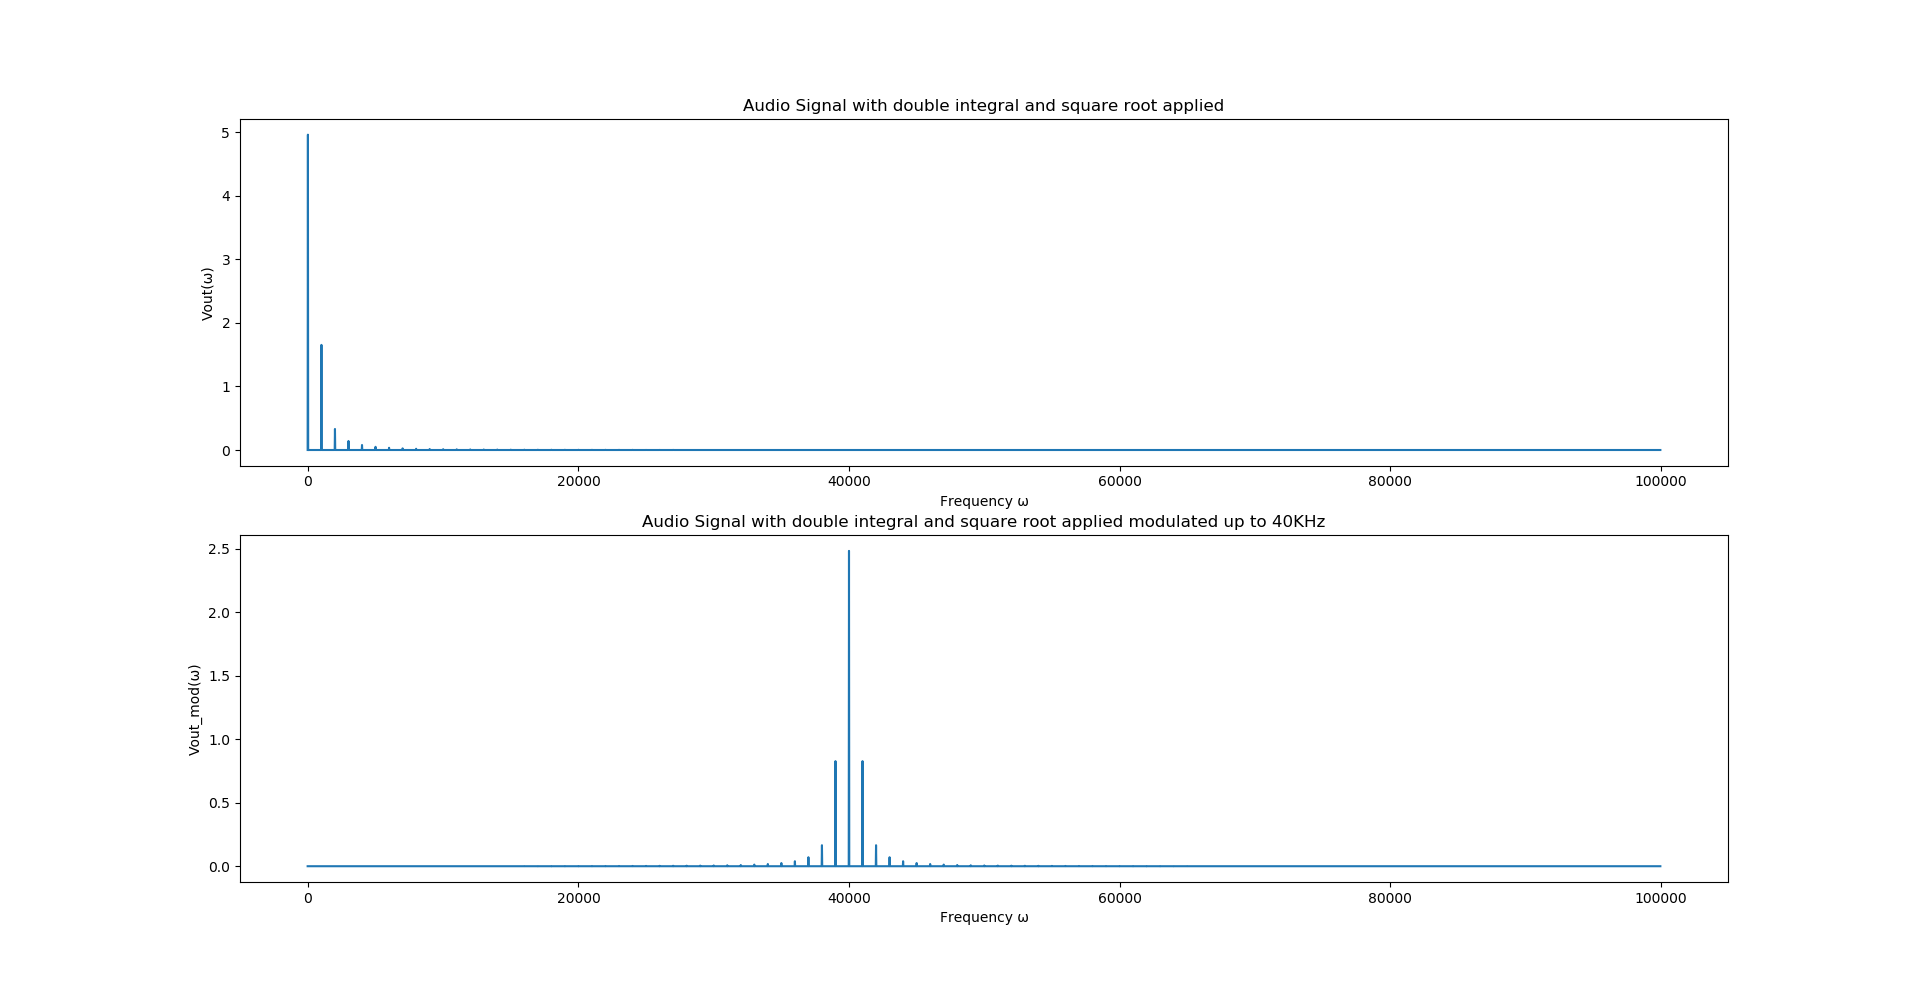
\includegraphics[width=0.8\textwidth]{Figures/SigSimulation/sqrt_sqrtmodfft.png}
    \caption{The frequency domain representation of the 1 kHz signal after the first and second integral}
    \label{fig:sqrtsimmodfft}
\end{figure}
The spectrums in figure \ref{fig:sqrtsimmodfft} show a large fundamental component with exponentially decaying harmonics. The fundamental along with its harmonics is then shifted up to 40 kHz without any aliasing. This result assumes that the bandwidth of the transducers are infinite and as such, are able to replicate all of these harmonics, however; this is not the case in practice. The bandwidth of the ultrasonic transducers is constrained to 2.5 kHz in the practical implementation since larger bandwidth transducers are impractical for a low cost implementation. This will result in imperfect inverse reproduction of the original signal when applied to the environment and likely result in deteriorated signal quality after demodulation.
\newpage
\subsubsection{Environment transfer function}
The output of the pre-processing simulation results in our processed signal modulated up to 40kHz. The environment then applies the mathematical operations from equation \ref{eqn:berktayRelationship} which starts with the squaring of the signal. Figure \ref{fig:sqrfilt} shows the result of squaring the modulated output (YOUT)  from the pre-processing simulation as well as the FIR filter described in listing \ref{lst:FIRfilter} along with the result from applying this filter. The result of the squaring of the signal is not immediately apparent and has been artificially amplified in figure \ref{fig:sqrfiltamp} to demonstrate where the frequency components of the signal now lie.
\begin{figure}[ht!]
    \centering
    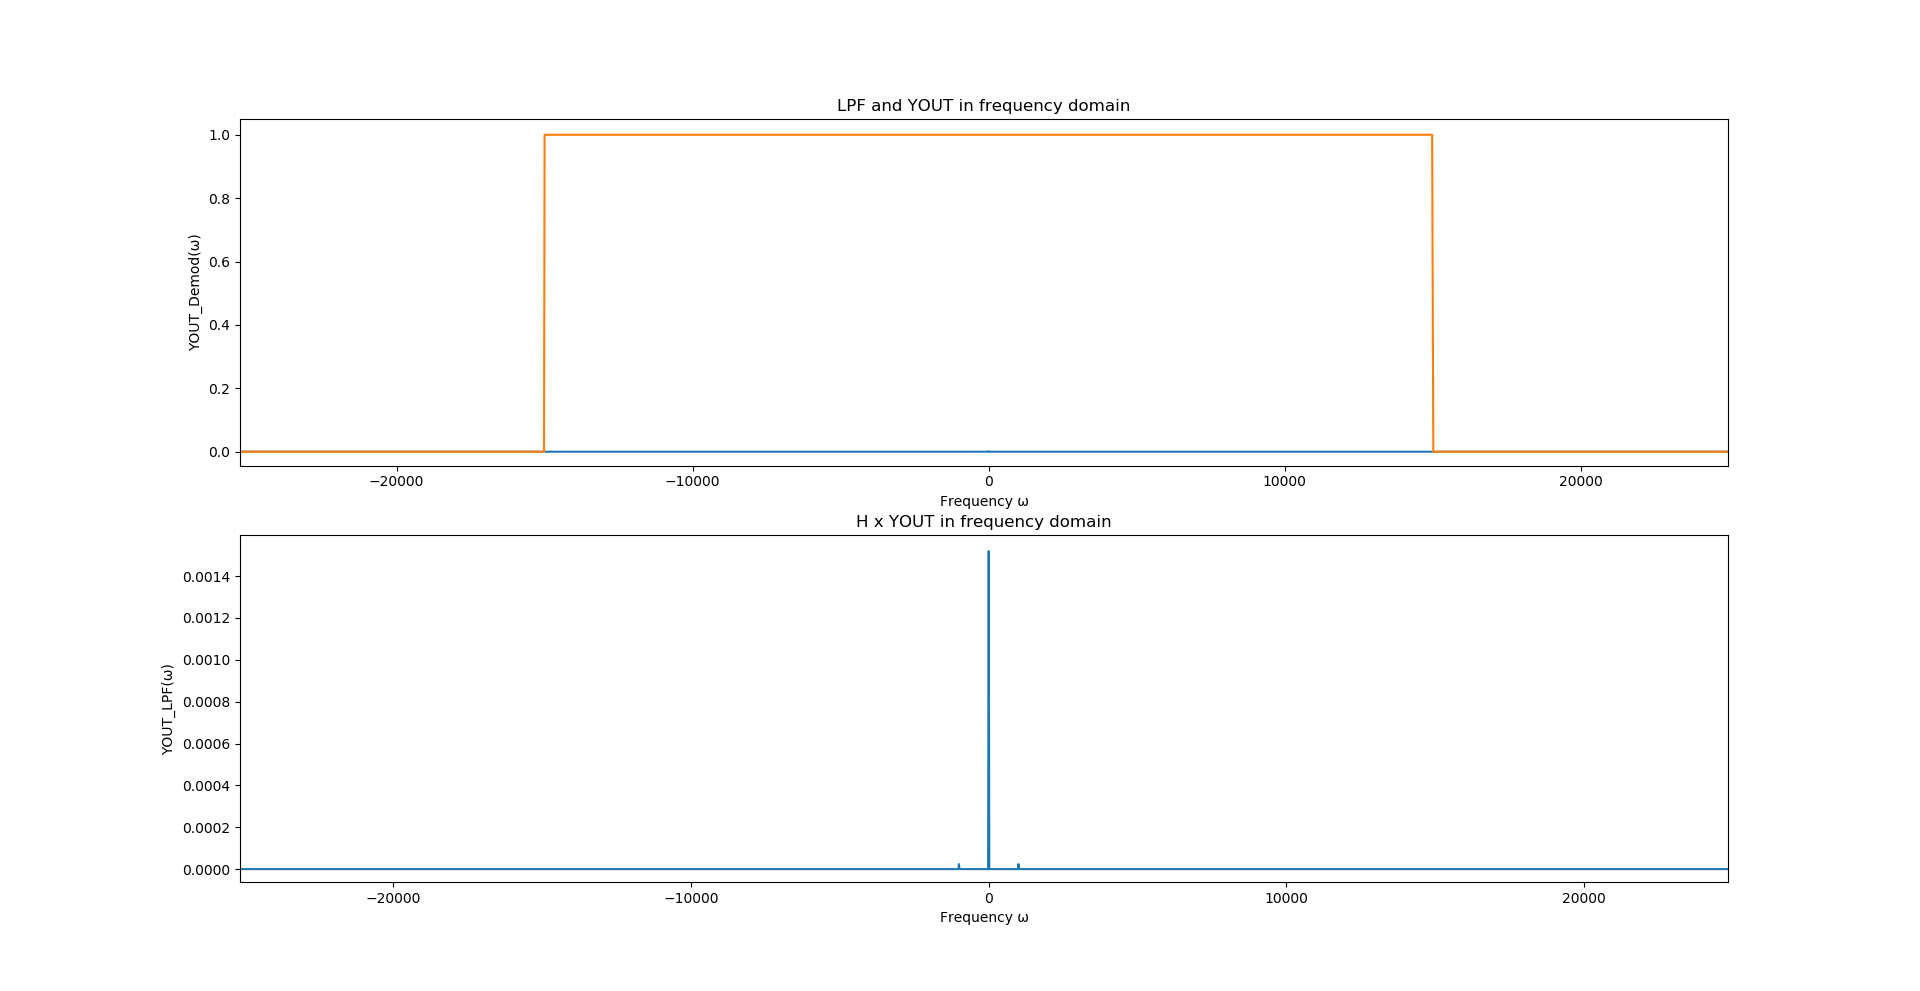
\includegraphics[width=0.8\textwidth]{Figures/SigSimulation/yRxsqr_LPFfft.png}
    \caption{The frequency domain representation of the 1 kHz signal after squaring, the FIR filter and the result of the filter.}
    \label{fig:sqrfilt}
\end{figure}

\begin{figure}[ht!]
    \centering
    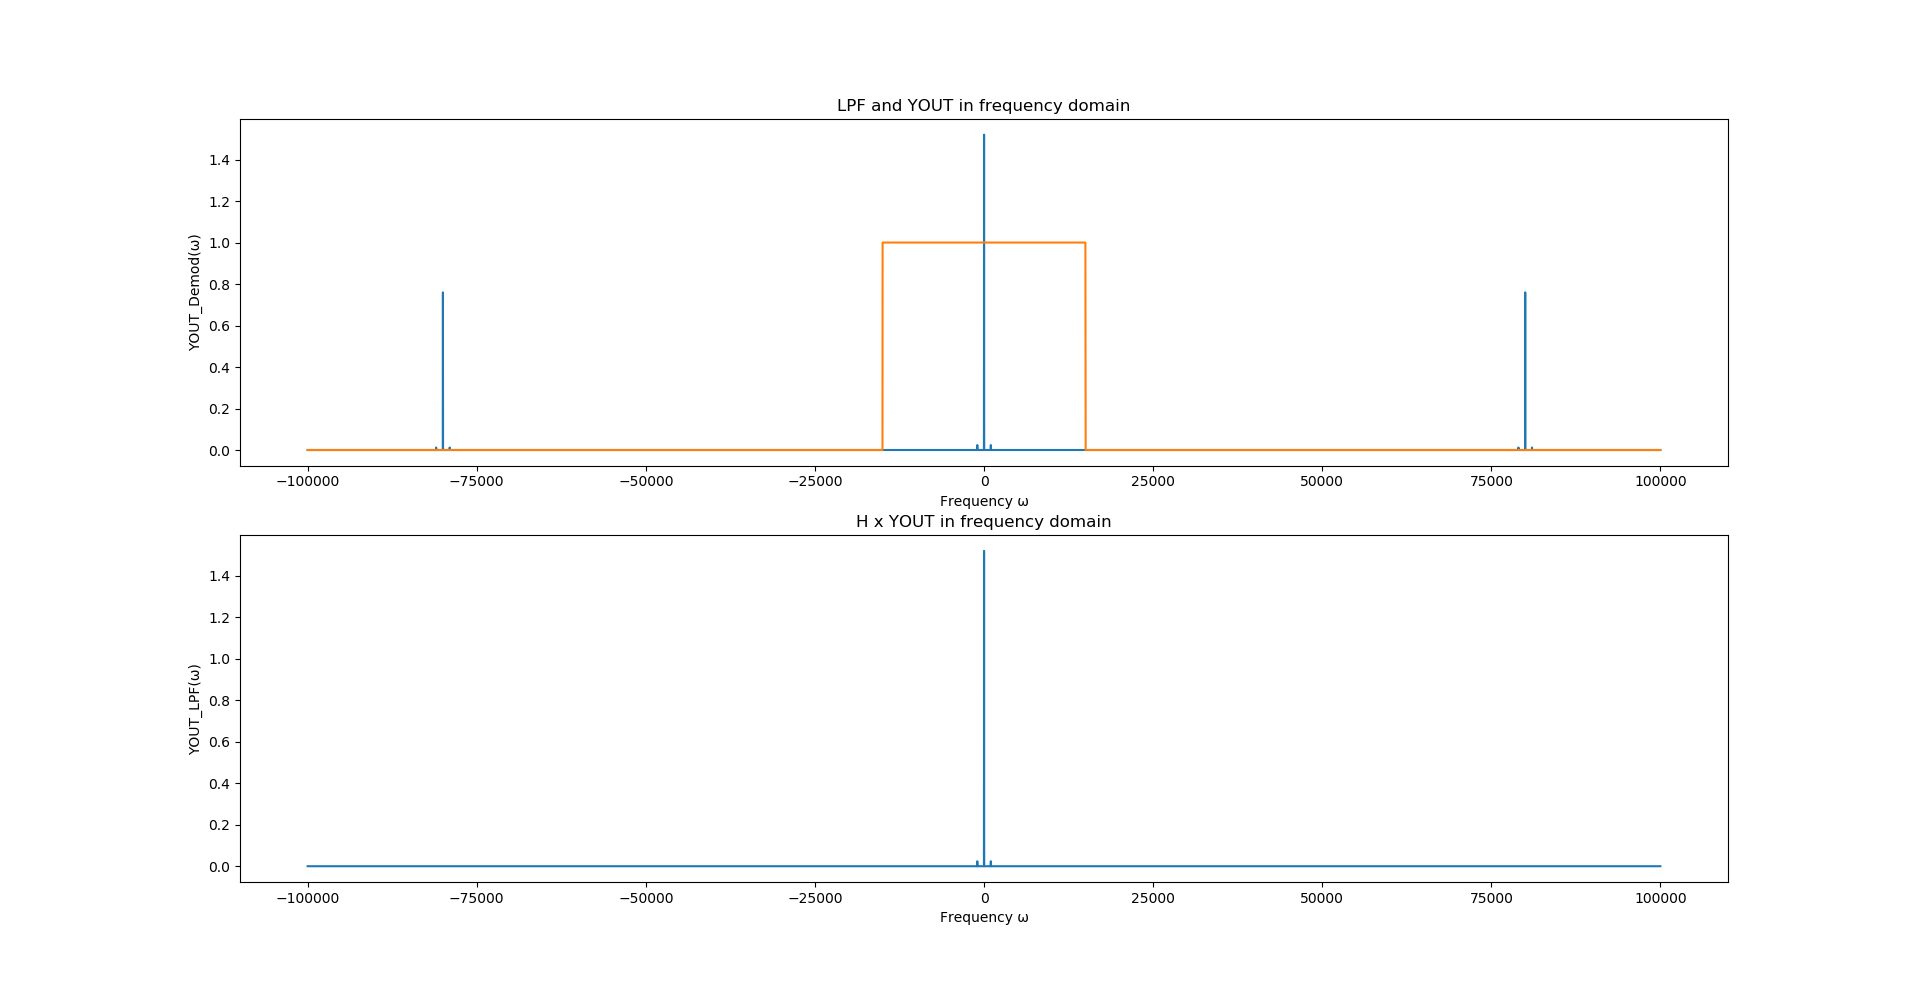
\includegraphics[width=0.8\textwidth]{Figures/SigSimulation/yRxsqr_LPFfftAmp1000.png}
    \caption{The frequency domain representation of the 1 kHz signal after squaring and amplification, the FIR filter and the result of the filter.}
    \label{fig:sqrfiltamp}
\end{figure}
The amplified signal in figure \ref{fig:sqrfiltamp} shows sum and difference frequencies at 80 kHz and baseband respectively. Upon application of the filter, only baseband signals are shown. A closer at the base band spectrum is shown in figure \ref{fig:sqrcrop} which represents a strong low frequency component with very small 1 kHz components.
\begin{figure}[ht!]
    \centering
    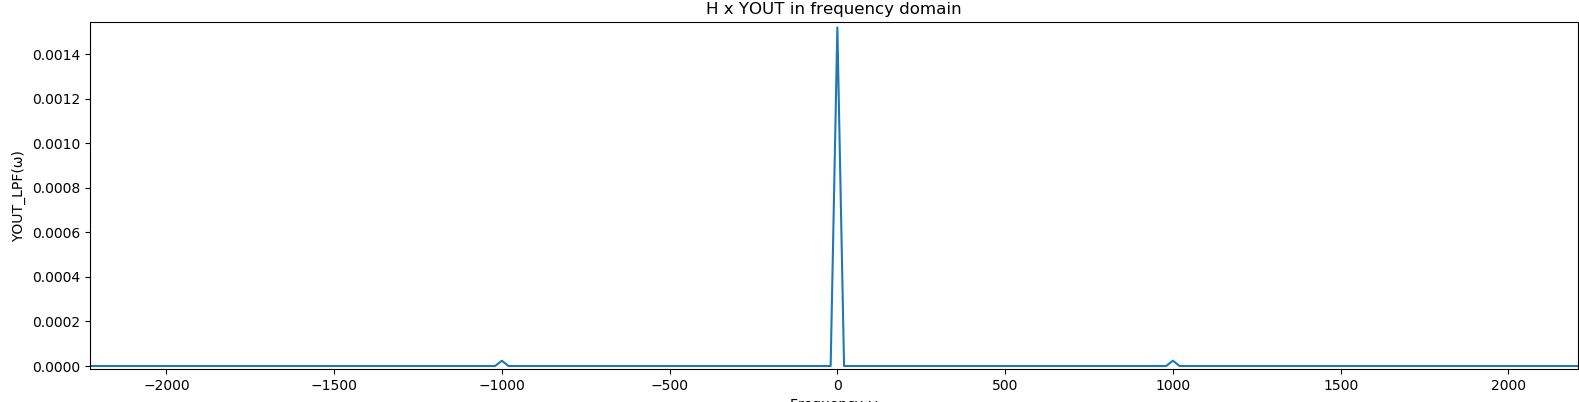
\includegraphics[width=0.8\textwidth]{Figures/SigSimulation/cropzoomedinyRxfilt.png}
    \caption{The frequency domain representation of the 1 kHz signal after squaring and filtering magnified between 0 and 2.5 kHz}
    \label{fig:sqrcrop}
\end{figure}

The next function the environment applies to the signal is a double derivative as described in listing \ref{lst:deriv}. The results from the first and second derivative are shown in figure \ref{fig:dt12simfft}.
The derivatives appear to amplify the low amplitude 1kHz components while effectively cancelling out the low frequency baseband signal acquired from the difference pair in the squaring process. By the application of the second derivative, the relative magnitude of the signal is significantly stronger.
\begin{figure}[ht!]
    \centering
    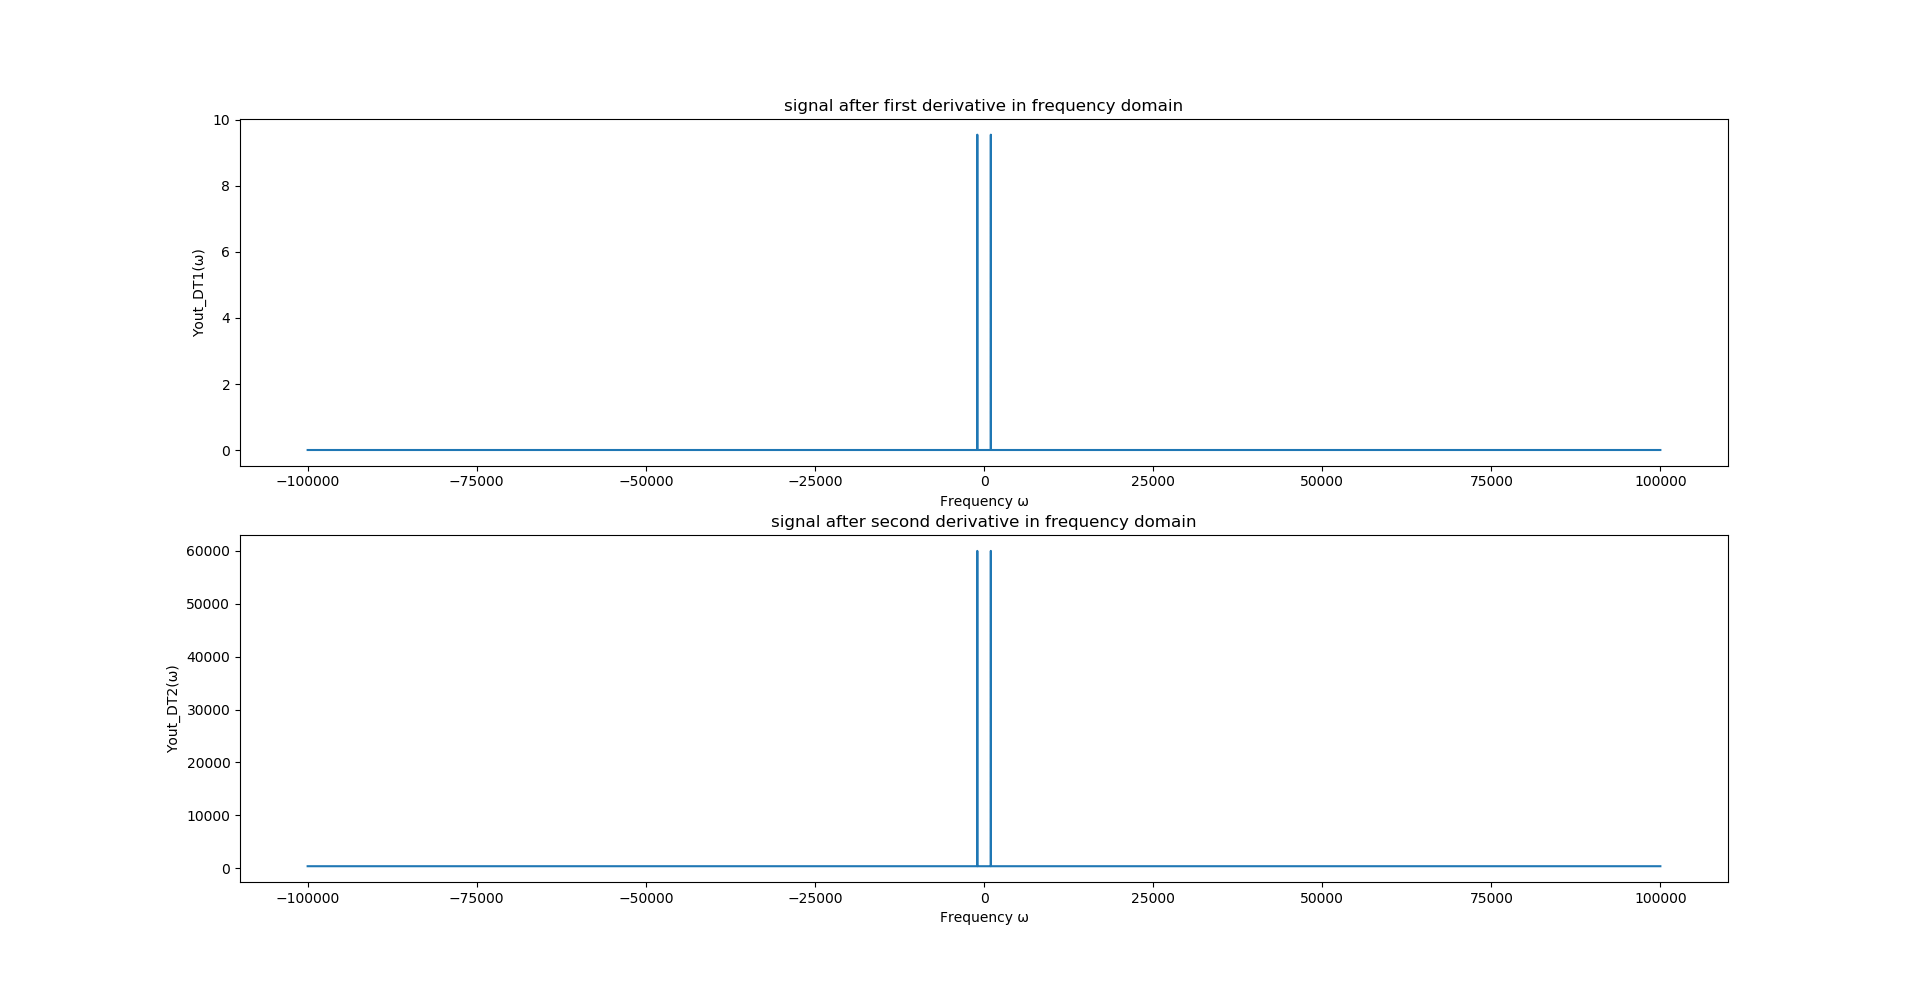
\includegraphics[width=0.8\textwidth]{Figures/SigSimulation/dt1dt2fft.png}
    \caption{The frequency domain representation of the 1 kHz signal after first and then second derivatives}
    \label{fig:dt12simfft}
\end{figure}
\newpage
The time domain representations of each derivative is compared to the original 1 kHz signal in figure \ref{fig:dt_tdom} where the output of the first and second derivatives are in blue and the original signal (scaled for easier comparison) is in orange. 
\begin{figure}[ht!]
    \centering
    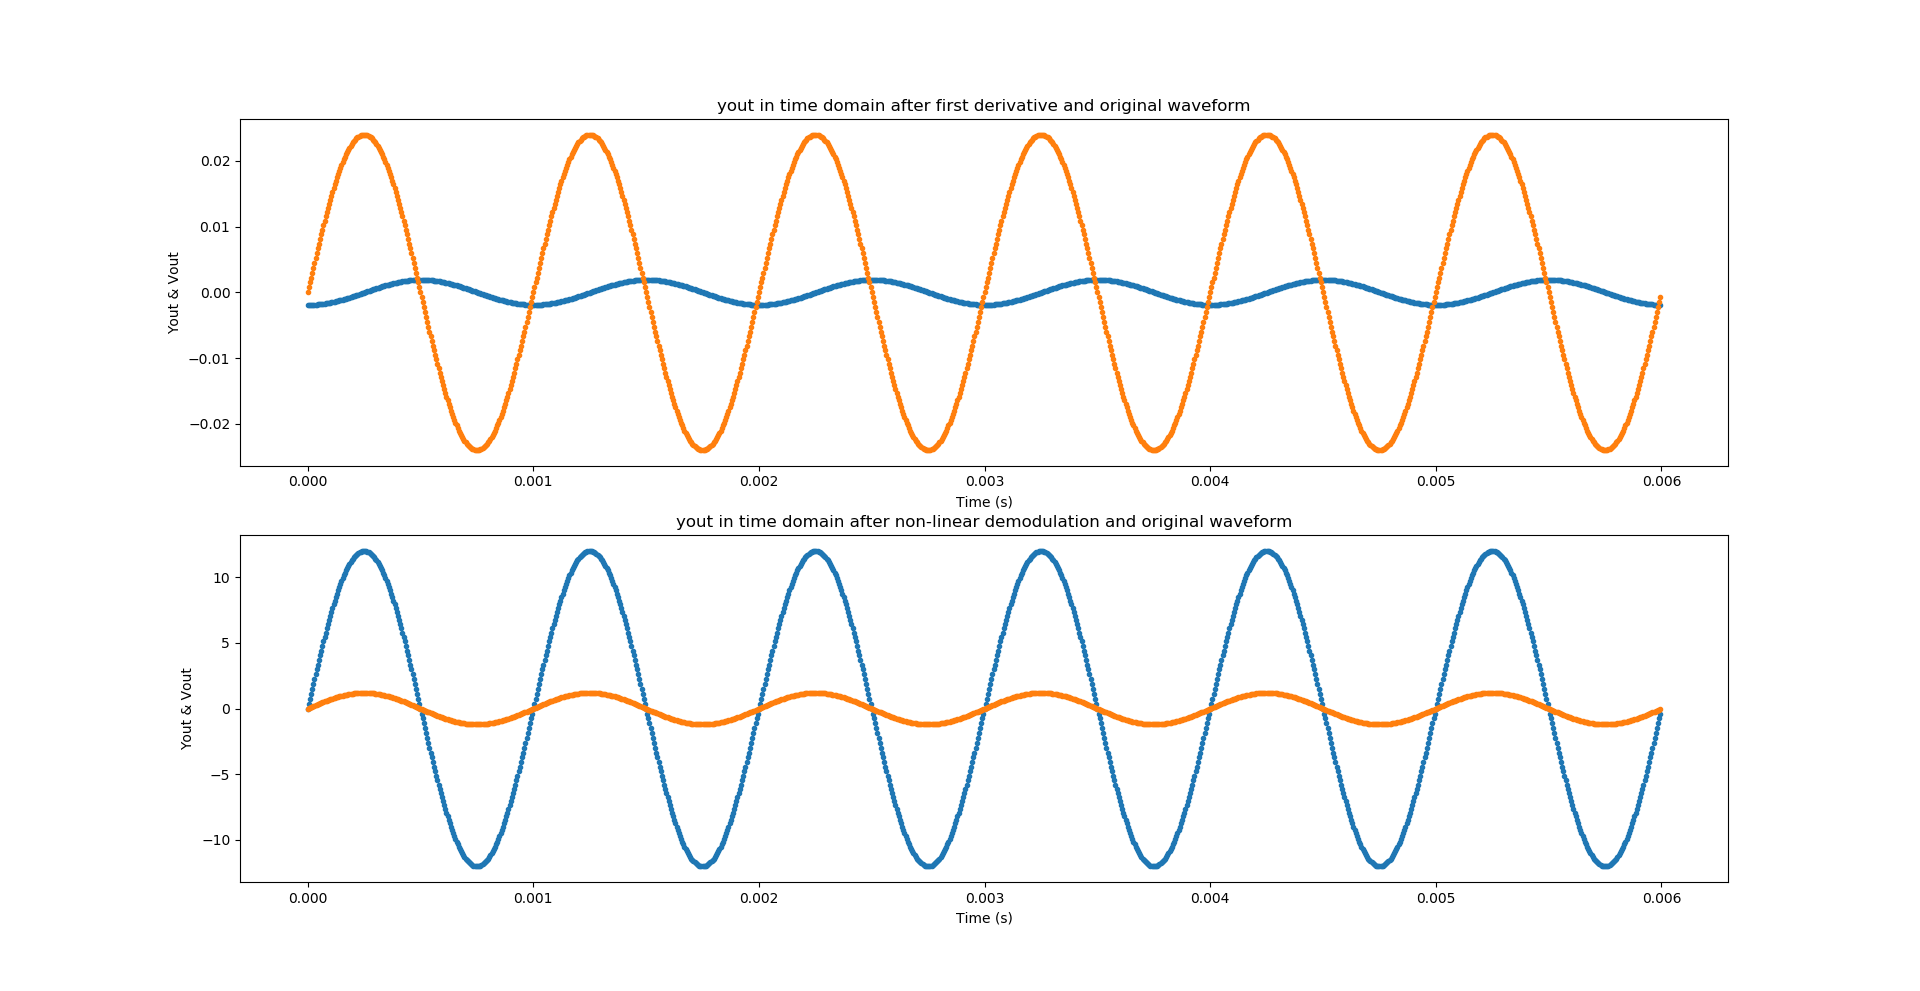
\includegraphics[width=0.8\textwidth]{Figures/SigSimulation/dt1vorig1div500_dt2vorig1div10.png}
    \caption{The time domain representation of the 1 kHz signal after first and then second derivatives (blue) compared to a scaled representation of the original 1kHz function (orange)}
    \label{fig:dt_tdom}
\end{figure}
Notably, the signal after the first derivative is out of phase with the original by $90^\circ$. However; after the second derivative the phases match. This is expected behaviour since the derivative of a sinusoidal function is that function again, shifted in phase by $90^\circ$.\\
Finally, to analyse the sample by sample representation of the output; figure \ref{fig:youtfinal} is plotted without any modification to the original signals amplitude nor phase.
\begin{figure}[ht!]
    \centering
    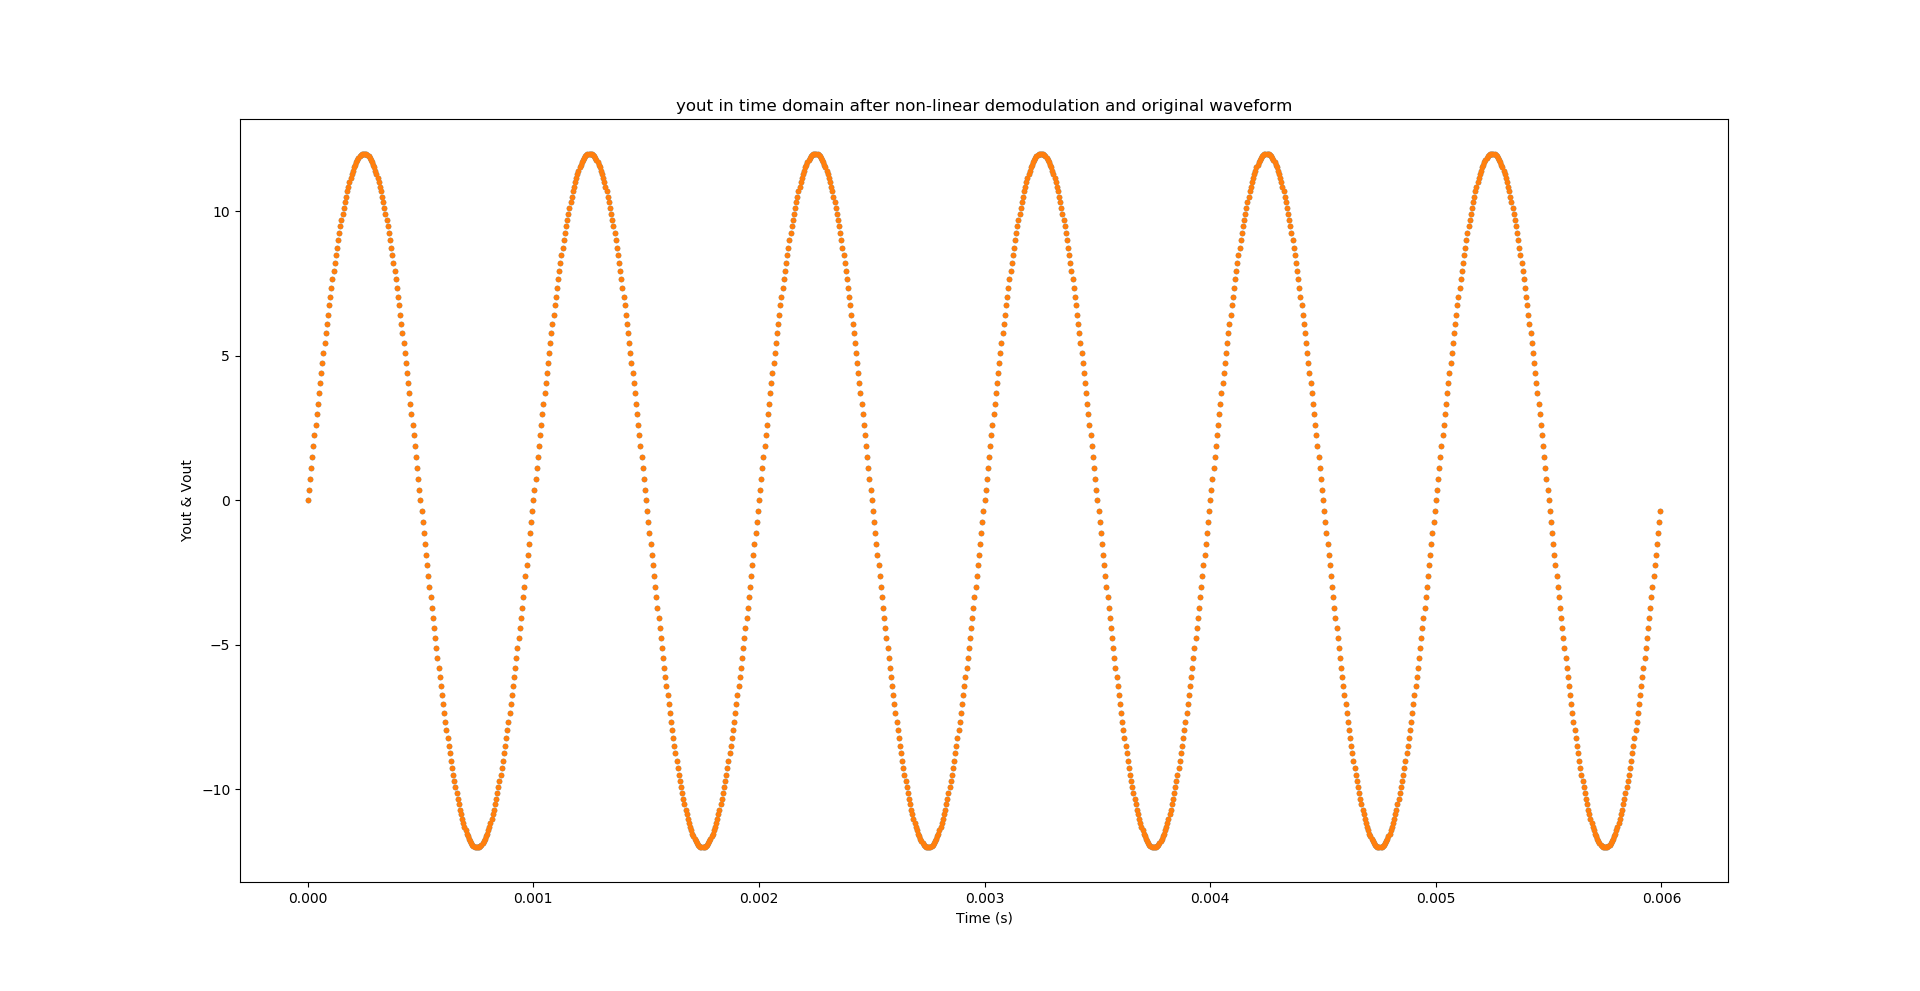
\includegraphics[width=0.8\textwidth]{Figures/SigSimulation/youtfulldemod.png}
    \caption{The time domain representation of the 1 kHz signal after passing through the environmental transfer function simulator (blue) compared with the original 1 kHz function (orange)}
    \label{fig:youtfinal}
\end{figure}
\newpage
Upon inspection, a sample for sample match of the input and output sinusoidal signals is achieved. This result demonstrates the full signal simulation was successful and all mathematical operations applied by the simulated environment were overcome with pre-processing.\\
While this result is expected in the theory and simulation, it remains unknown how the bandwidth limitations of the transducers will effect the output. The ultrasonic transducer's transfer function is not modelled nor is its frequency response as this is left to be a potential future improvement of the simulation for a future iteration of this project. This future iteration of the simulation might consider measuring the frequency response of the transducers and using this data to apply a filter to the 40 kHz AM output signal.
\subsection{Simulation complications}
During the initial implementation of the signal pre-processing and environment modelling stages, the discrete signal processing outputs were causing artifacts in the signal plots. This was caused by the \texttt{deriv()} functions in code listings \ref{lst:deriv}. The outputs of the derive function were discontinuous because the first sample of the input signal (\texttt{x[n-1]} where \texttt{n} is 1) is 0 while the first sample of the input signal (\texttt{x[n-1]} where \texttt{n} is 2) is a much larger number than 0. This discontinuity caused a large spike in the output of the function between the first two samples. Initially this was discovered by setting \texttt{y[1]=y[2]} which yeilded the correct output for a derivative of the input function. Later it was decided that the first sample of our signal didn't really hold much value due to the high number of samples in the sampled signal and the \texttt{shiftBackBy()} function was created to shift the signal back by a sample and thus, remove that first sample from the output.